\subsection{Aplica\c c\~ao}\label{subsec:estudo-reslt}


A previsão da demanda d'água é uma preocupação fundamental para muitas organizações e autoridades responsáveis pelo abastecimento d'água. Neste estudo de caso, explorou-se como a análise de séries temporais pode ser aplicada para prever a demanda d'água ao longo do tempo.


\subsubsection{Estudo de Caso 1 - An\'alise de Padr\~oes de Consumo}\label{subsubsec:quest-est}

\textbf{Questão de Pesquisa:} Existe tendência, padrão, sazonalidade para os dados destes três anos do Bairro Alto?
 
Na análise dos dados dos últimos 2 anos do Bairro Alto utilizando o método de decomposição STL mostrado na Figura \ref{fig:stl}, constatou-se que identificar tendências, sazonalidades e padrões de consumo d'água não é uma tarefa fácil. Essa dificuldade em compreender os dados torna-se um desafio na hora de planejar o abastecimento de forma eficiente.

O gráfico de barras apresentado na Figura \ref{fig:grafico-barras-demanda} mostra a demanda média das variáveis de fluxo (Vazão de Entrada -- FT01, Vazão de Gravidade -- FT02 e Vazão de Recalque -- FT03) durante o intervalo das 18h às 21h. Cada barra representa a média da demanda para cada variável em um horário específico dentro desse intervalo. A altura de cada barra indica a magnitude da demanda média para a respectiva variável. Essa visualização permite que seja identificado o horário em que as variáveis de fluxo apresentaram maior demanda, o que é útil para o planejamento e gerenciamento adequado do sistema.

\begin{figure}[!htb]
	\centering
	\caption{Demanda média das variáveis de fluxo.}
	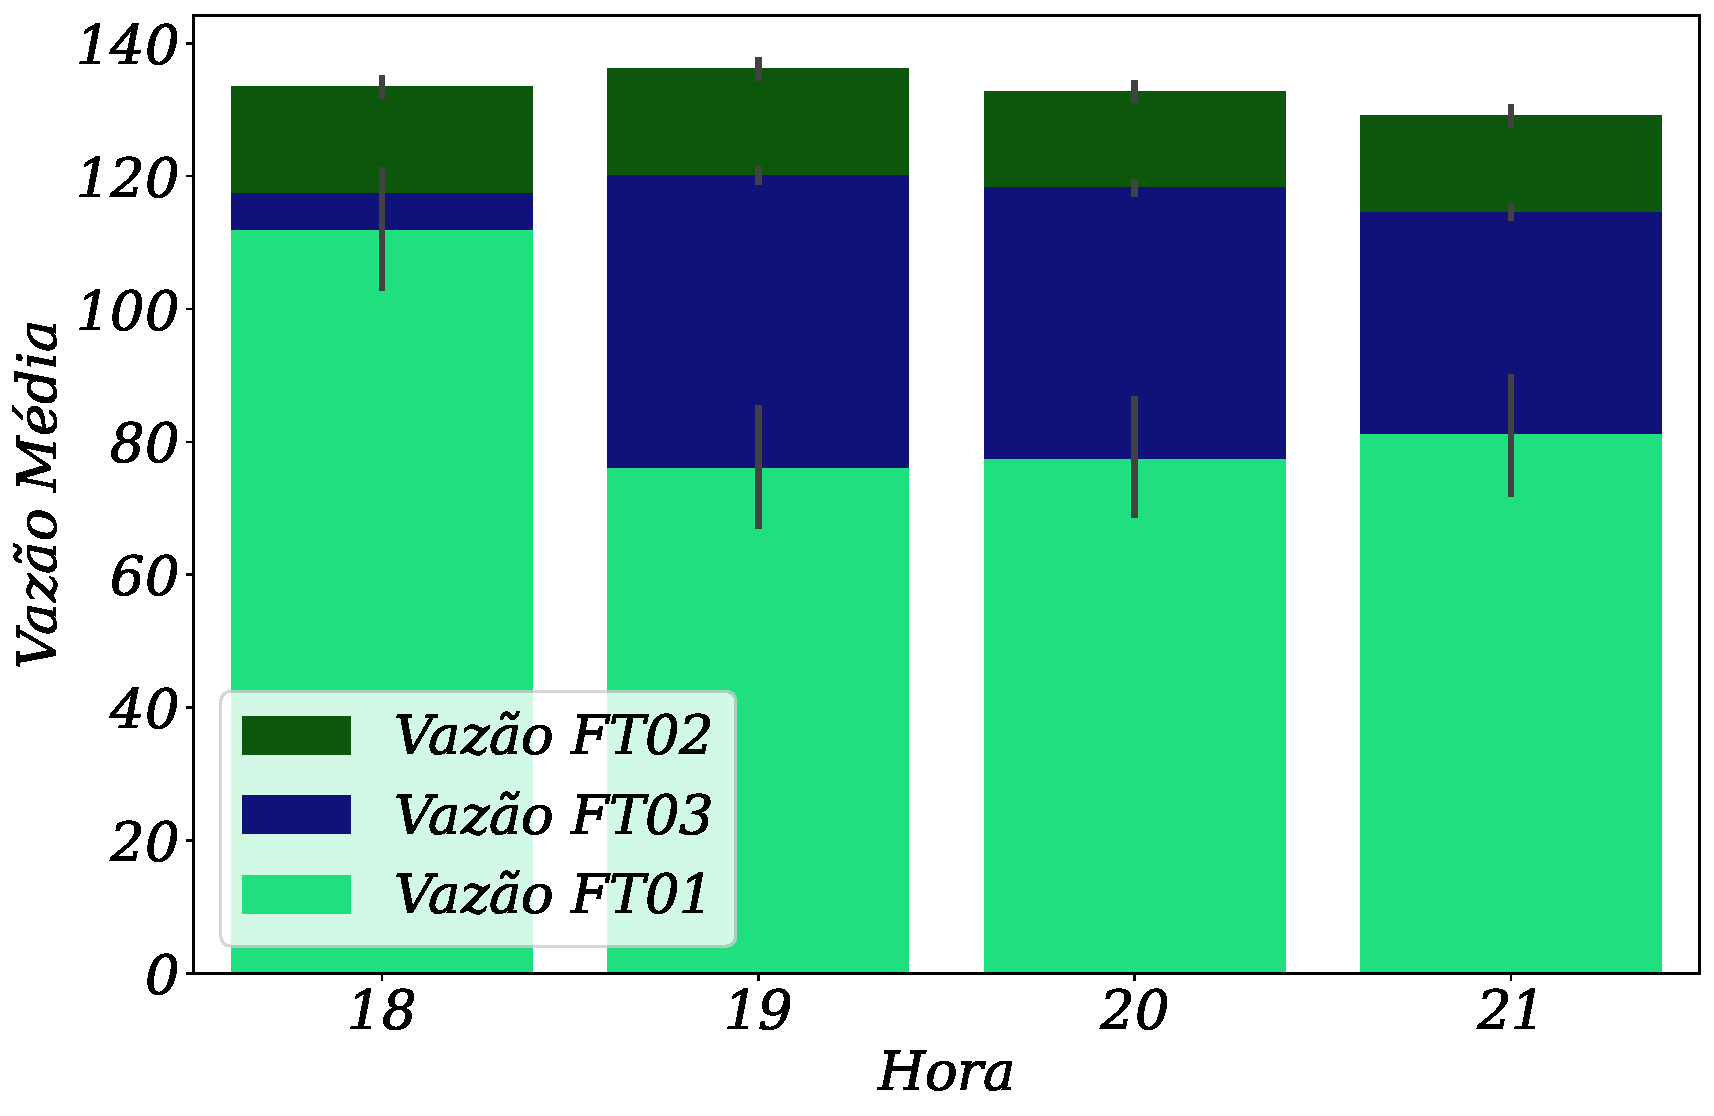
\includegraphics[width=0.7\linewidth]{Resultados/Figuras/grafico-barras-demanda}
	
	\label{fig:grafico-barras-demanda}
	
	
\end{figure}

\subsubsection{Estudo de Caso 2 -- Estrat\'egias de Economia de Energia}

\textbf{Questão de Pesquisa:} Qual é o impacto do acionamento das bombas durante o horário de pico?

Confirma-se que a ativação das bombas de sucção durante o período de 18h às 21h resulta em um maior custo energético para a SANEPAR. Portanto, é recomendado evitar o acionamento das bombas durante esse período, utilizando estratégias de armazenamento e gerenciamento eficientes.

\textbf{Questão de Pesquisa:} Qual é o nível ideal no reservatório para evitar a ativação das bombas da SANEPAR durante o período de maior demanda, das 18h às 21h, sem comprometer o abastecimento d'água para a população?

Verifica-se que, para evitar o acionamento das bombas durante o horário de pico (18h às 21h) sem comprometer o abastecimento d'água para a população, é necessário manter o nível do reservatório acima de $4.445$ litros.


A Tabela \ref{tb:dem} apresenta os resultados para as três variáveis estudadas: vazão de entrada -- FT01, vazão de gravidade -- FT02 e vazão de recalque -- FT03. Os resultados destacam os horários específicos em que cada variável apresentou maior demanda dentro do intervalo das 18h às 21h, fornecendo importantes informações para o planejamento e gerenciamento adequado do sistema.



\begin{table}[!htb]
	\centering
	\caption{Demanda d'água.}\label{tb:dem}
	\begin{tabular}{@{}lll@{}}
		\toprule
		\textbf{Vazões}         & \textbf{Horário de Maior Demanda} & \textbf{Demanda} \\ \midrule
		Entrada -- FT01   & 2020/10/08 21:00:00               & $383,87 \ m^3/h$                   \\
		Gravidade -- FT02 & 2020/10/20 18:00:00               & $326,17 \ m^3/h$                    \\
		Recalque -- FT03  & 2020/11/26 19:00:00               & $194,35 \ m^3/h$                    \\ \bottomrule
	\end{tabular}
	
	
\end{table}

Durante as horas de pico, é necessário que o nível do reservatório esteja mantido dentro na média de $4.445$ litros para evitar o acionamento das bombas. Manter o nível do reservatório dentro dessa faixa permitirá que o sistema opere de forma eficiente, atendendo à demanda d'água sem a necessidade de acionar as bombas.

É importante destacar que a vazão de recalque exerce um impacto significativo no nível do reservatório em comparação com as outras vazões. Essa diferença se deve ao fato de que a vazão de recalque está diretamente relacionada à injeção d'água no reservatório por meio da bomba localizada próxima à sua base. Em contraste, as demais vazões possuem alguns valores ausentes, o que limita sua influência na análise geral do sistema.
